% DO NOT COMPILE THIS FILE DIRECTLY!
% This is included by the other .tex files.
\section*{Background}
\begin{frame}[t,plain]
\titlepage
\end{frame}
%%%%%%%%%%%%%%%%%%%%%%%%%%%%%%%%%%%
%%%%%%%%%%%%%%%%%%%%%%%%%%%%%%%%%%%
\begin{frame}{Combining (expert) opinions}
\begin{figure}
 \begin{center}
  
\includegraphics[scale=0.5]{figures/Consensus.jpg}
 \end{center}
\end{figure}
\end{frame}
%%%%%%%%%%%%%%%%%%%%%%%%%%%%%%%%%%%
%%%%%%%%%%%%%%%%%%%%%%%%%%%%%%%%%%%
\begin{frame}{Logarithmic pooling -- Definition \& Notation}
Let $\mathbf{F_\theta} = \{f_0(\theta), f_1(\theta), \ldots, f_K(\theta)\}$ be the set of \sout{prior} distributions representing the opinions of $K+1$ experts and let $\boldsymbol\alpha =\{\alpha_0, \alpha_1, \ldots, \alpha_K \}$ be the vector of weights, such that $\alpha_i > 0\: \forall i$ and $\sum_{i=0}^K \alpha_i = 1$.
Then the log-pooled prior is
\begin{equation}
\label{eq:logpool}
 \mathcal{LP}(\mathbf{F_\theta}, \boldsymbol\alpha) := \pi(\theta \mid \boldsymbol\alpha) = t(\boldsymbol\alpha) \prod_{i=0}^K f_i(\theta)^{\alpha_i}, 
\end{equation}
where the normalising term $t(\boldsymbol\alpha) = \int_{\boldsymbol\Theta}\prod_{i=0}^K f_i(\theta)^{\alpha_i}d\theta$ is guaranteed to exist for all proper $f_i$.
We simplify the proof given by~\cite{genest1986A} by using H\"{o}lder's inequality.
This operator enjoys a number of desirable properties such as external Bayesianity~\citep{genest1986A}, relative propensity consistency~\citep{genest1984} and log-concavity~\citep{Carvalho2019}.
\end{frame}
%%%%%%%%%%%%%%%%%%%%%%%%%%%%%%%%%%%
%%%%%%%%%%%%%%%%%%%%%%%%%%%%%%%%%%%
\begin{frame}{Logarithmic pooling -- Properties}
\begin{property}
\label{prp:EB}
 \textbf{External Bayesianity~\citep{genest1984}}. Combining the set of posteriors $p_i(\theta \mid x) \propto  l(x \mid \theta)f_i(\theta) $ yields the same distribution as combining the densities $f_i$ to obtain a prior $\pi(\theta)$ and then combine it with $l(x \mid \theta)$ to obtain a posterior $p(\theta \mid x) \propto l(x \mid \theta)\pi(\theta)$.
\end{property}

\begin{property}
\label{prp:concavity}
\textbf{Log-concavity}. 
 Let $\mathbf{F}_{\theta}$ be a set of log-concave distributions, i.e., each $f_i$ can be written as $ f_i(\theta) \propto e^{\nu_i(\theta)}$, where $\nu_i(\cdot)$ is a concave function.
Then $\pi(\theta\mid \boldsymbol \alpha)$ is also log-concave.
\end{property}
\end{frame}
%%%%%%%%%%%%%%%%%%%%%%%%%%%%%%%%%%%
%%%%%%%%%%%%%%%%%%%%%%%%%%%%%%%%%%%
\begin{frame}{Logarithmic pooling -- more properties}
\begin{property}
\label{prp:RPC}
\textbf{Relative propensity consistency~\citep{genest1984}}.
Taking $\boldsymbol F_{X}$ as a set of expert opinions with support on a space $\mathcal{X}$, define $\boldsymbol \xi = \{\boldsymbol F_{X}, a, b\}$ for arbitrary $a , b \in \mathcal{X}$.
Let $\mathcal{T}$ be a pooling operator and define two functions $U$ and $V$ such that 
\begin{align}
 U(\boldsymbol \xi) &:= \left( \frac{f_0(a)}{f_0(b)}, \frac{f_1(a)}{f_1(b)}, \ldots, \frac{f_K(a)}{f_K(b)} \right)\:\text{and}\\
 V(\boldsymbol \xi) & := \frac{\mathcal{T}_{\boldsymbol F_{X}} (a)}{\mathcal{T}_{\boldsymbol F_{X}} (b)}.
\end{align}
We then say that $\mathcal{T}$ enjoys \textit{relative propensity consistency} (RPC) if and only if
\begin{equation}
 U(\boldsymbol \xi_1) \geq U(\boldsymbol \xi_2) \implies  V(\boldsymbol \xi_1) \geq V(\boldsymbol \xi_2),
\end{equation}
for all $\boldsymbol \xi_1, \boldsymbol \xi_2$.
\end{property}

\begin{itemize}
 \item Properties~\ref{prp:EB} and~\ref{prp:RPC} are~\textbf{unique} to logarithmic pooling.
\end{itemize}

\end{frame}
%%%%%%%%%%%%%%%%%%%%%%%%%%%%%%%%%%%
%%%%%%%%%%%%%%%%%%%%%%%%%%%%%%%%%%%
\begin{frame}{Weights are crucial}
The weights $\boldsymbol\alpha$ are key to the shape and properties of the combined (pooled) distribution.
\begin{itemize}
 \item In theory, the weights should reflect the~\textit{reliabilities} of the experts/information sources;\pause
 \item In practice, reliabilities are hard to determine;\pause
 \item As we will see, combining probability distributions in particular can lead to counterintuitive results.\pause
\end{itemize}
Here we will consider three ways of constructing the weights ``objectively'': 
\begin{itemize}[label=\ding{212}]
 \item Maximise the entropy of $\pi$;\pause
 \item Minimise the Kullback-Leibler divergence between $\pi$ and each $f_i$;\pause
 \item Place a probability measure over $\boldsymbol\alpha$.
\end{itemize}
 \end{frame}
%%%%%%%%%%%%%%%%%%%%%%%%%%%%%%%%%%%
%%%%%%%%%%%%%%%%%%%%%%%%%%%%%%%%%%%
\begin{frame}{Maximise the entropy of $ \pi(\theta)$ }
 \begin{itemize}
  \item If there is no information about the reliabilities of the experts one might want to construct $\boldsymbol\alpha$ so as to maximise entropy of the resulting distribution:
  \begin{align*}
   H_{\pi}(\theta) &=-\int_{\boldsymbol\Theta}\pi(\theta)\ln\pi(\theta)d\theta \\
   H_{\pi}(\theta; \boldsymbol\alpha) &= -\sum_{i=0}^{K} \alpha_i E_{\pi}[\log f_i] - \log t(\boldsymbol\alpha).
  \end{align*}
  \item Formally, we want to find $\hat{\boldsymbol\alpha}$ such that
  \[\hat{\boldsymbol\alpha}:= \argmax H_{\pi}(\theta; \boldsymbol\alpha)  \]
  \item Caveats: (i) is not guaranteed to yield an unique solution; (ii) is rather prone to yield ``degenerate'' (trivial) solutions.
 \end{itemize}
\end{frame}
%%%%%%%%%%%%%%%%%%%%%%%%%%%%%%%%%%%
%%%%%%%%%%%%%%%%%%%%%%%%%%%%%%%%%%%
\begin{frame}{Minimise KL divergence between $\pi(\theta)$ and the $f_i$'s}
\begin{itemize}
 \item What if we want to minimise conflict between the consensus and each individual opinion?
 \item Let $d_i = \text{KL}(\pi || f_i)$ and let $L(\boldsymbol\alpha)$ be a loss function such that
\begin{align*}
L(\boldsymbol\alpha) &= \sum_{i=0}^Kd_i \\
     &=  - (K+1) \sum_{i=0}^K\alpha_i\mathbb{E}_\pi [\log f_i ]  - \sum_{i=0}^K \mathbb{E}_\pi\left[\log f_i\right] - \log t(\boldsymbol\alpha), \\
     \hat{\boldsymbol\alpha}:=& \argmin L(\boldsymbol\alpha)   
\end{align*}
\item Contrary to the maximum entropy problem, the loss function is convex, thus there is a unique solution~\citep{rufo2012A}.
\end{itemize}
\end{frame}
%%%%%%%%%%%%%%%%%%%%%%%%%%%%%%%%%%%
%%%%%%%%%%%%%%%%%%%%%%%%%%%%%%%%%%%
\begin{frame}{Place a prior on the weights}
 \begin{itemize}
  \item An appealing alternative is to place a (hyper) prior on the weights ($\boldsymbol\alpha$);
  \item Two approaches:\\
 (a) Dirichlet prior:
\[ \pi_A(\boldsymbol\alpha \mid \boldsymbol X) = \frac{1}{\mathcal{B}(\boldsymbol X)}\prod_{i=0}^K \alpha_i^{x_i-1}.\]
 (b) logistic-normal:
 \begin{align*}
  &\pi_A(\boldsymbol\alpha \mid \boldsymbol \mu, \boldsymbol \Sigma) = \frac{1}{|2\pi \boldsymbol \Sigma|^{\frac{1}{2}}}\frac{1}{\prod_{i=0}^K \alpha_i}
  \exp\left(
     \left(\boldsymbol \eta - \boldsymbol \mu\right)^T
     {\boldsymbol \Sigma}^{-1}
     \left( \boldsymbol \eta - \boldsymbol \mu\right)
     \right),\\
      &\boldsymbol \eta := \log\left(\frac{\boldsymbol \alpha_{-K}}{\alpha_K}\right).
 \end{align*}
 \item Advantage: accomodates uncertainty in natural way, and is very flexible;
 \item Caveat(s): may yield inconsistent results and hardly ever allows for analytical solutions for the marginal prior $g(\theta) = \int_{\mathcal{A}} \pi(\theta \mid \boldsymbol\alpha)d\Pi_A$.
 \end{itemize}
\end{frame}
%%%%%%%%%%%%%%%%%%%%%%%%%%%%%%%%%%%
%%%%%%%%%%%%%%%%%%%%%%%%%%%%%%%%%%%
\begin{frame}{Priors on the weights: details}
 \begin{itemize}
\item Match the first two moments of the Logistic-normal to the Dirichlet~\citep{aitchson1980}:
  \begin{align*}
 \label{eq:momentmatching}
 \mu_i & = \psi(x_i) - \psi(x_K), \quad i=0,1,\ldots,K-1, \\
 \Sigma_{ii} & = \psi'(x_i) + \psi'(x_K), \quad i=0,1,\ldots,K-1, \\
 \Sigma_{ij} & = \psi'(x_K),
\end{align*}
where $\psi(\cdot)$ is the digamma function, and $\psi'(\cdot)$ is the trigamma function.
\item Exploit a non-centering trick to sample from the logistic normal~\textit{via} Cholesky decomposition of $\boldsymbol \Sigma$;  
\item We explore two sets of hyperparameters: $\boldsymbol X = \{1, 1, \ldots, 1\}$ and $\boldsymbol X^\prime = \boldsymbol X/10$;
 \end{itemize}
\end{frame}
%%%%%%%%%%%%%%%%%%%%%%%%%%%%%%%%%%%
%%%%%%%%%%%%%%%%%%%%%%%%%%%%%%%%%%
\begin{frame}{Application: survival probabilities (reliability)}
 \begin{itemize}
  \item \cite{savchuk1994} consider an example in which four experts are required supply prior information about the survival probability of
a certain unit for which there have been $y = 9$ successes out of $n = 10$ trials;
  \item $Y\sim Bernoulli(\theta)$ and
  \[f_i(\theta;a_i, b_i) = \frac{\Gamma(a_i + b_i)}{\Gamma(a_i b_i)} \theta^{a_i-1}(1-\theta)^{b_i-1}\]
  \item Allows for simple expressions for the entropy and KL divergence [$\pi(\theta; \boldsymbol\alpha)$ is also Beta], and efficient sampling from the hyperpriors; 
  \item For this example, we can evaluate performance using integrated (marginal) likelihoods, a.k.a., prior evidence.
 \end{itemize}
\end{frame}
%%%%%%%%%%%%%%%%%%%%%%%%%%%%%%%%%%%
%%%%%%%%%%%%%%%%%%%%%%%%%%%%%%%%%%%
\begin{frame}{Survival probabilities: results}
\begin{figure}[!ht]
\begin{center}
\subfigure[][Expert priors]{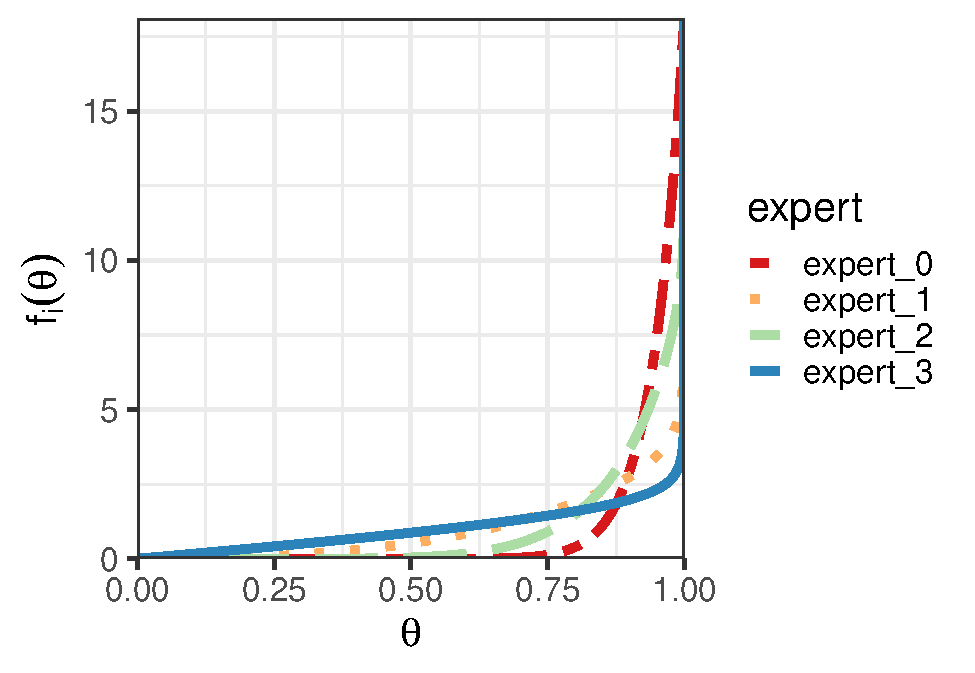
\includegraphics[scale=.22]{../plots/expert_densities_Savchuk.pdf}}
\subfigure[][Pooled priors]{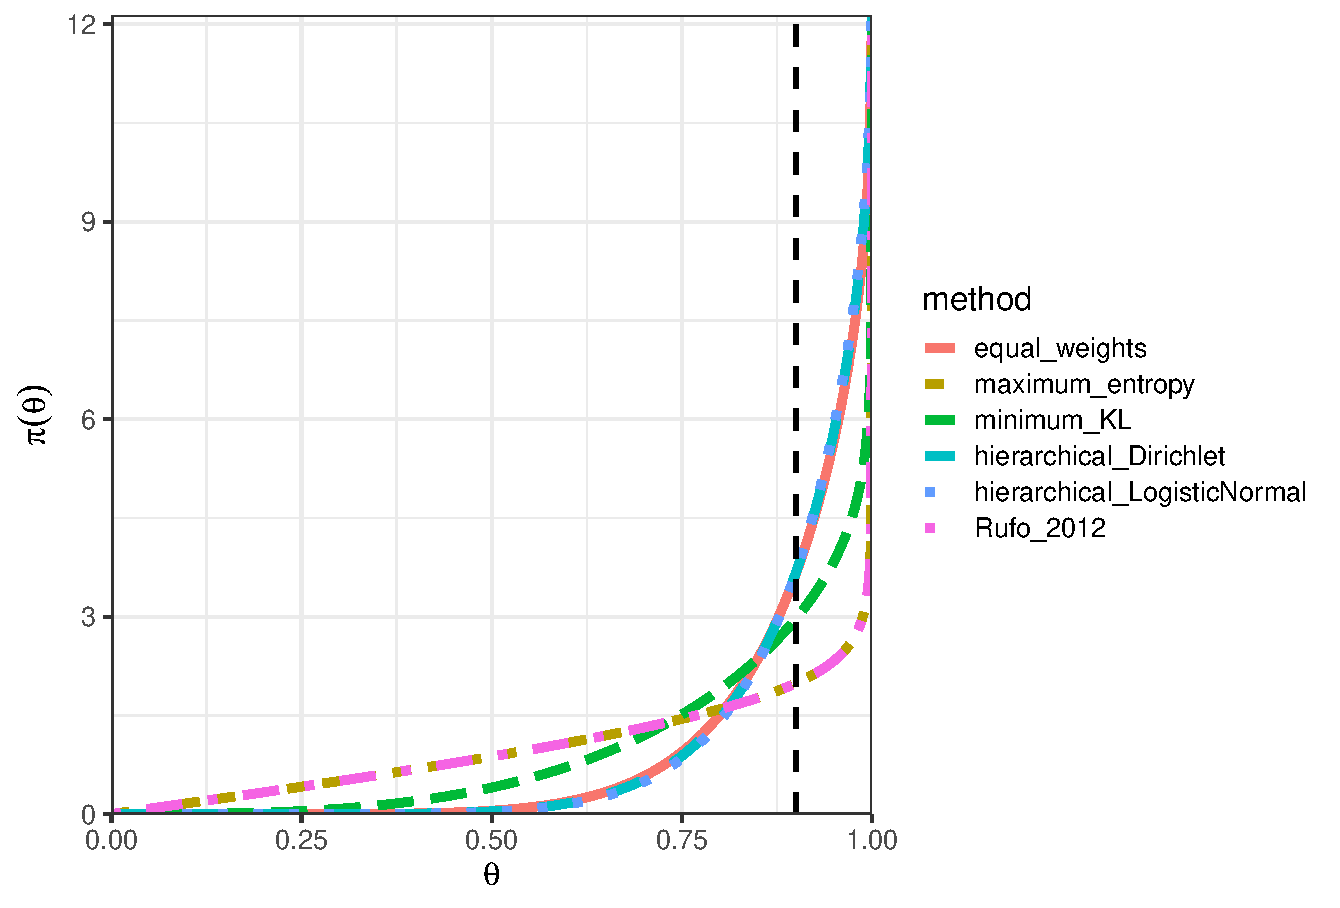
\includegraphics[scale=.22]{../plots/method_prior_densities_Savchuk.pdf}}
\end{center}
\label{fig:priors_pooled_Savchuk}
\end{figure}
\end{frame}
%%%%%%%%%%%%%%%%%%%%%%%%%%%%%%%%%%%
%%%%%%%%%%%%%%%%%%%%%%%%%%%%%%%%%%%
\begin{frame}{Survival probabilities: results II}
\begin{table}[ht]
\centering
\begin{tabular}{ccccc}
  \hline
Method  & $\alpha_0$ & $\alpha_1$ & $\alpha_2$ & $\alpha_3$ \\ 
  \hline
Maximum entropy & 0.00 & 0.00 & 0.00 & 1.00 \\ 
Minimum KL divergence & 0.04 & 0.96 & 0.00 & 0.00 \\
\cite{rufo2012A} & 0.00 & 0.00 & 0.00& 1.00\\
Dirichlet prior & 0.26 & 0.24 & \textcolor{blue}{\textbf{0.27}} & 0.23 \\ 
Logistic-normal prior & 0.27 & 0.24 & \textcolor{blue}{\textbf{0.31}} & 0.18\\
 \hline
\end{tabular}
\label{tab:alphasBeta}
\end{table}
\begin{table}[ht]
\centering
\begin{tabular}{cccc}
   \hline
   \multicolumn{2}{c}{Expert priors} &  \multicolumn{2}{c}{Pooled priors} \\
   \hline
   Expert 0 & 0.237 & Equal weights & 0.254\\
   Expert 1 & 0.211 & Maximum entropy & 0.163 \\
   Expert 2 & \textcolor{blue}{\textbf{0.256}} & Minimum KL & 0.223 \\ 
   Expert 3 & 0.163 & Hierarchical prior (Dirichlet/logistic-normal) & \textcolor{blue}{\textbf{0.255}} \\
   \hline
\end{tabular}
\label{tab:marglikes}
\end{table}
\end{frame}
%%%%%%%%%%%%%%%%%%%%%%%%%%%%%%%%%%%
%%%%%%%%%%%%%%%%%%%%%%%%%%%%%%%%%%%
\begin{frame}{Simulated example: can we reliably learn the weights?}
Setup:  Five experts elicit Beta priors on a quantity $p$. Data will be $x/n = 5/10$. Only expert 2 (let's call her Mãe Diná) gives a reasonable prior with mean $\mu_2 = 0.50$ and coefficient of variation $c_2$.
\begin{figure}[!ht]
\begin{center}
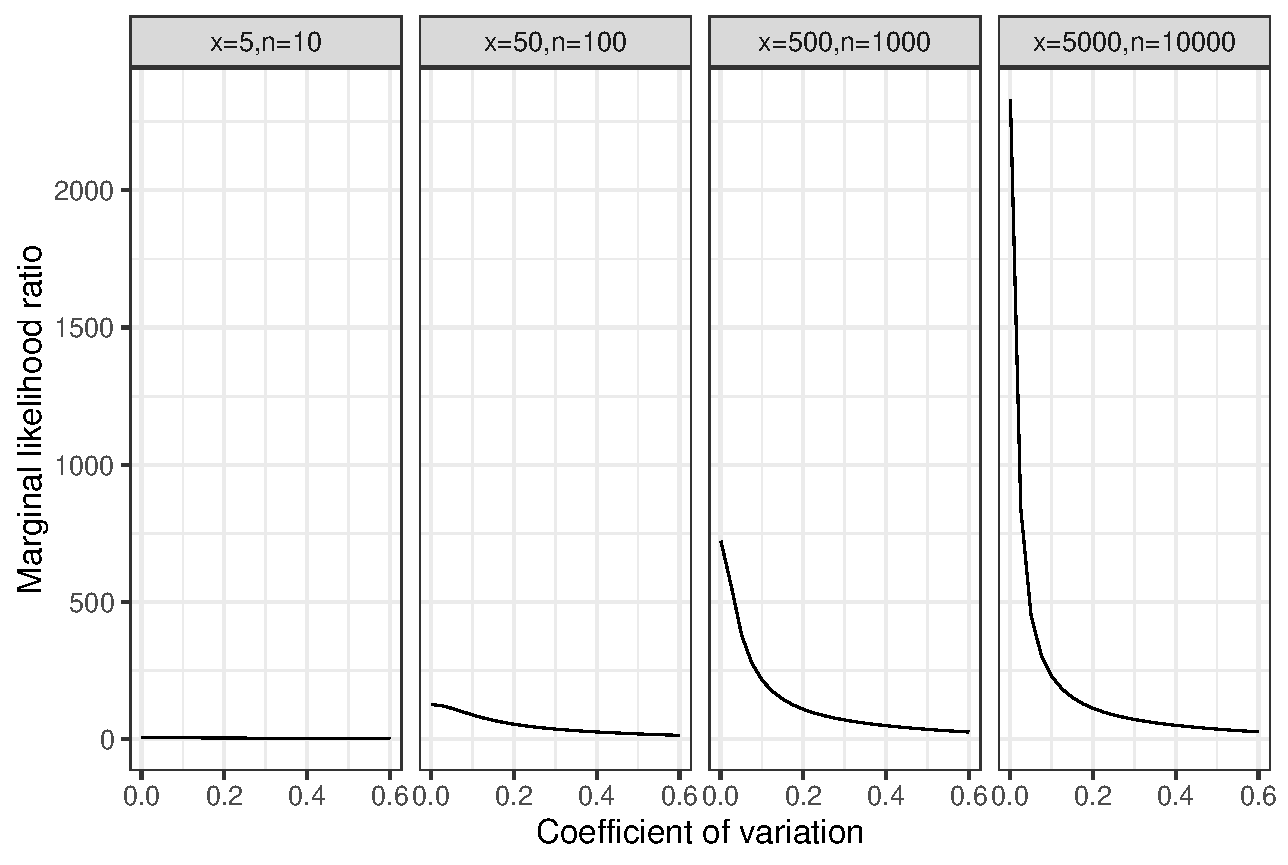
\includegraphics[scale=.40]{../plots/MaLs_ratios_oneCorrect.pdf}
\end{center}
\label{fig:one_correct_marglikes}
\end{figure}
\end{frame}
%%%%%%%%%%%%%%%%%%%%%%%%%%%%%%%%%%%
%%%%%%%%%%%%%%%%%%%%%%%%%%%%%%%%%%%
\begin{frame}{Simulated example: performance of hierarchical priors}
\begin{figure}[!ht]
\begin{center}
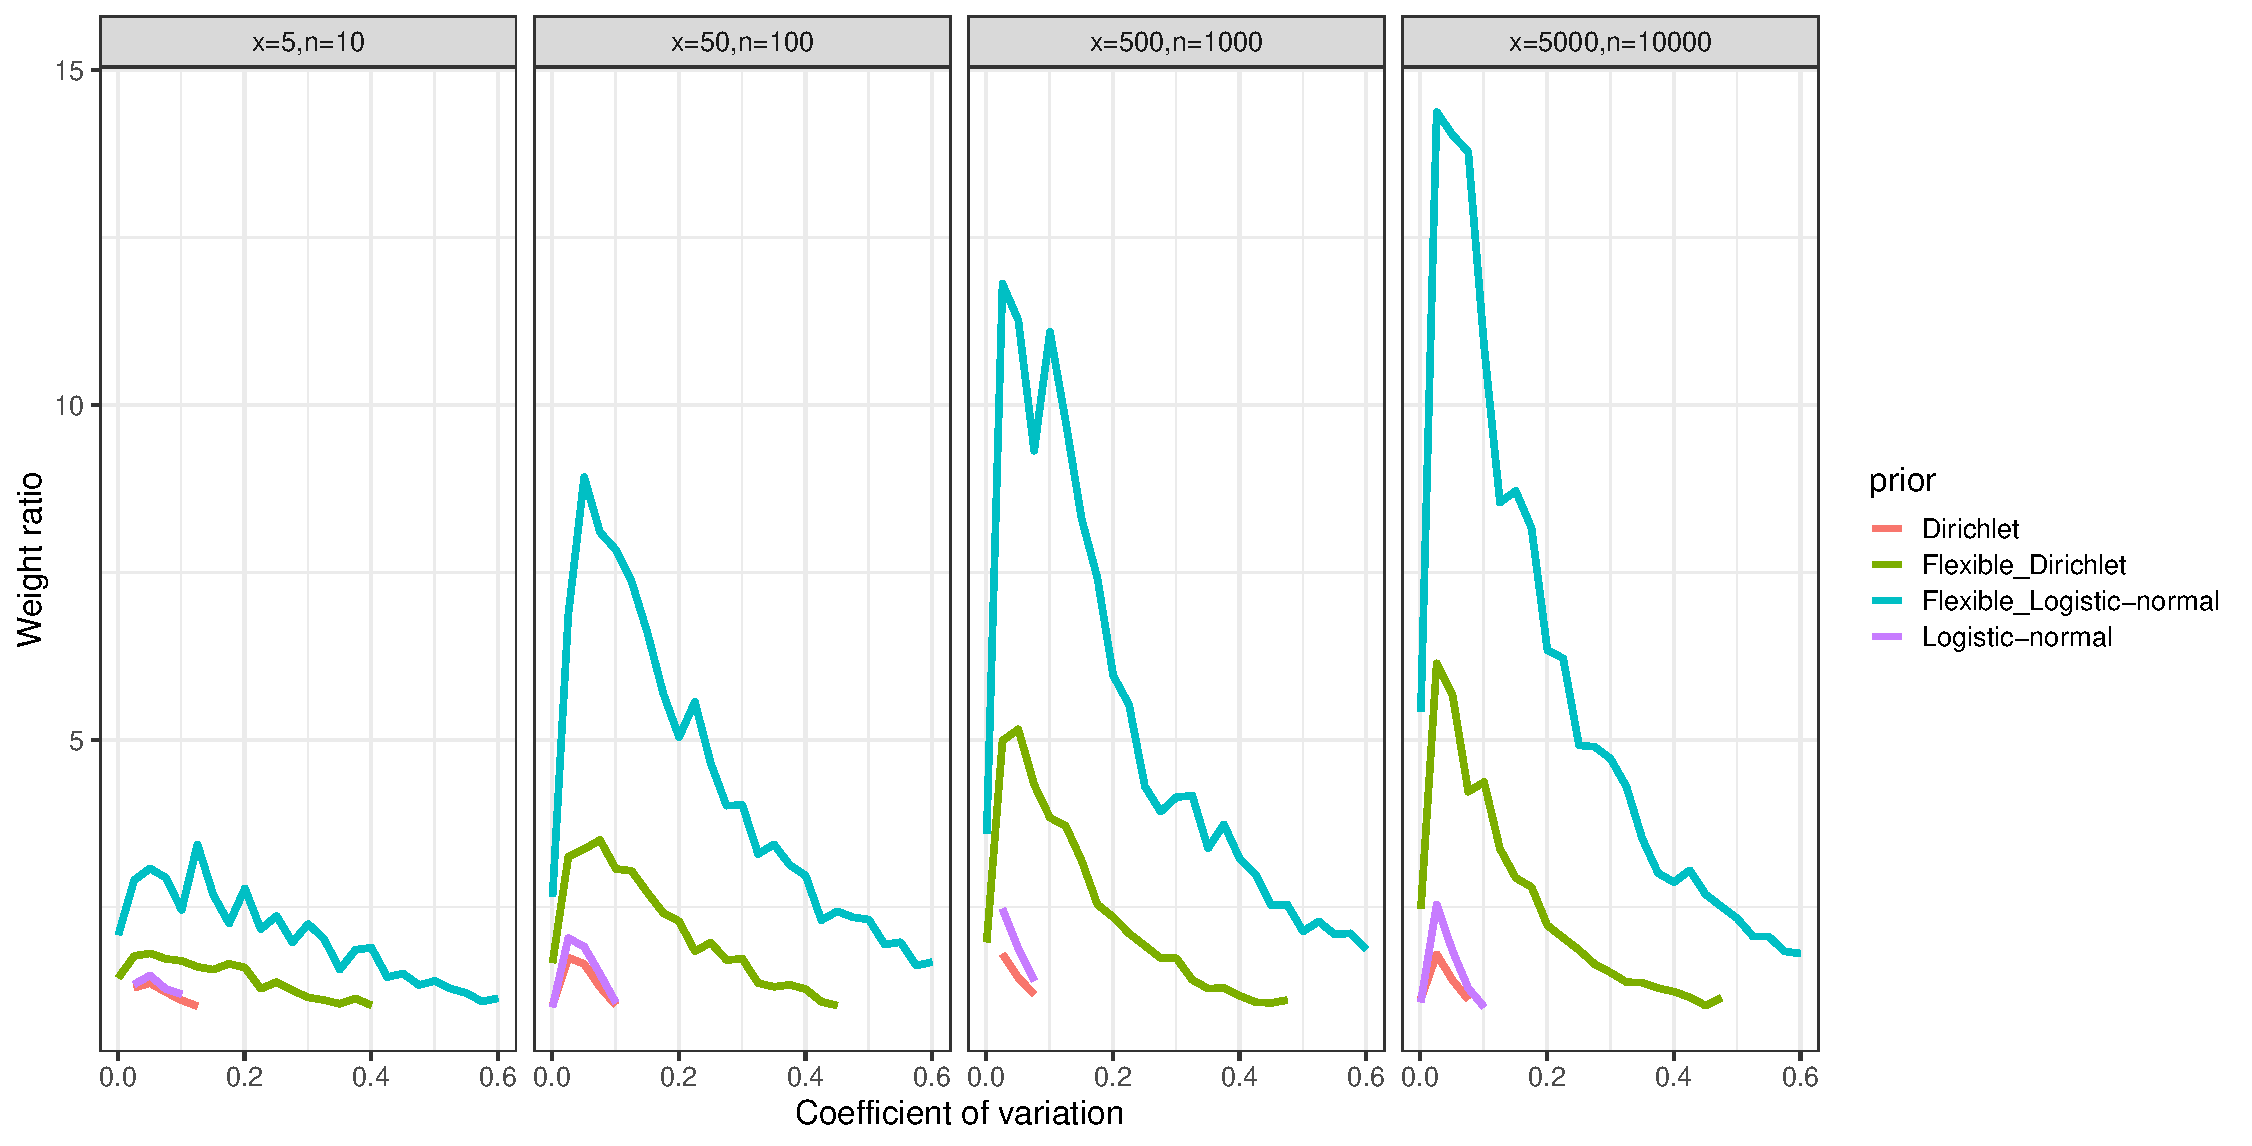
\includegraphics[scale=.30]{../plots/weight_ratios_oneCorrect.pdf}
\end{center}
\label{fig:one_correct_posteriors}
\end{figure}
\end{frame}
%%%%%%%%%%%%%%%%%%%%%%%%%%%%%%%%%%%
%%%%%%%%%%%%%%%%%%%%%%%%%%%%%%%%%%%
\begin{frame}{Simulated example: explaining the weirdness}
\begin{itemize}
 \item Let $c_2 = 0.2$ and $c_j = 0.1$ for all $j \neq 2$, with $\boldsymbol\mu = \{0.1, 0.2, \mathbf{0.5}, 0.8, 0.9\}$;\pause
 \item This setup leads to $\boldsymbol a = \{ 89.9, 79.8, \mathbf{12.0}, 19.2, 9.1\}$ and $\boldsymbol b = \{809.1, 319.2, \mathbf{12.0}, 4.8, 1.01\} $;\pause
 \item If the data are $x = 5$ and $n = 10$, computing marginal likelihoods and normalising would lead to weights $\boldsymbol\alpha^{\prime\prime} = \{0.006, 0.095, \mathbf{0.710}, 0.142, 0.048\}$;\pause
 \item However, by calculating $a^{\star\star} = \sum_{i = 0}^K \alpha_i^{\prime\prime} a_i = 19.75$ and $b^{\star\star} =  \sum_{i = 0}^K \alpha_i^{\prime\prime} b_i = 44.00$, we obtain a pooled prior with $\mathbb{E}_\pi [p] =  0.31$, far off the ``optimal'' $1/2$;\pause
 \item If the data were, say, $x = 50, n = 100$, then one would obtain a pooled prior for which $\mathbb{E}_\pi [p] = 0.51$.\pause
 \item [\textcolor{red}{\textbullet}] \textcolor{red}{Let $c_2 = 0.001$. Then $a_2 = b_2 = 499999.5$. Can you see the problem?}
\end{itemize}
\end{frame}
%%%%%%%%%%%%%%%%%%%%%%%%%%%%%%%%%%%
%%%%%%%%%%%%%%%%%%%%%%%%%%%%%%%%%%%
\begin{frame}{Inference of deterministic models via Bayesian melding}
\begin{center}
\textbf{Bayesian melding} 
\end{center}
Suppose we have deterministic model $M$ with inputs $\theta \in \boldsymbol\Theta \subseteq \mathbb{R}^p$ and outputs $\phi \in \boldsymbol\Phi\subseteq \mathbb{R}^q$, such that $\phi = M(\theta)$.
We have the combined prior on the outputs:
\begin{equation}
 \label{eq:BMpoolprior}
 \tilde{q}_{\Phi}(\phi) \propto q_1^\ast(\phi)^\alpha q_2(\phi)^{1-\alpha},
\end{equation}
where $q_1^\ast()$ is the \textbf{induced} and $q_2$ is ``natural'' prior on $\phi$.
The prior in~(\ref{eq:BMpoolprior}) can then be inverted to obtain a \textit{coherised} prior on $\theta$, $\tilde{q}_{\Theta}(\theta)$.
Standard Bayesian inference may then follow,  leading to the posterior
\begin{equation}
 \label{eq:BMpoolposterior}
 p_{\Theta}(\theta \mid \boldsymbol y, \alpha) \propto \tilde{q}_{\Theta}(\theta) L_1(\theta) L_2(M(\theta))\pi_A(\alpha).
\end{equation}
\end{frame}
%%%%%%%%%%%%%%%%%%%%%%%%%%%%%%%%%%%
%%%%%%%%%%%%%%%%%%%%%%%%%%%%%%%%%%%

\begin{frame}{Application: Influenza in a boarding school}
In 1978, $512$ out of $763$ lads got came down with the flu.
We model the spread using a standard SIR model
\begin{eqnarray*}
\frac{dS}{dt}&=& - \beta SI,\\
\frac{dI}{dt}&=&  \beta SI - \gamma I,\\
\frac{dR}{dt}&=& \gamma I, 
\end{eqnarray*} 
where  $S(t) + I(t) + R(t) = N \: \forall t$, $\beta$ is the transmission (infection) rate and $\gamma$ is the recovery rate.
The basic reproductive number is 
\begin{equation}
\label{eq:r0def}
R_0 = \frac{\beta N}{\gamma}. 
\end{equation}
We choose $\beta, \gamma \sim \text{log-normal}(0, 1)$ ($q_1$) and $R_0 \sim  \text{log-normal}(\mu_2, \sigma_2)$ such that $R_0$ has a mean of $1.5$ and a standard deviation of $0.25$ ($q_2$) which is informed by seasonal flu. 
\end{frame}
%%%%%%%%%%%%%%%%%%%%%%%%%%%%%%%%%%%
%%%%%%%%%%%%%%%%%%%%%%%%%%%%%%%%%%%
\begin{frame}{SIR model: results}
\begin{figure}[!ht]
\begin{center}
\subfigure[][$R_0$]{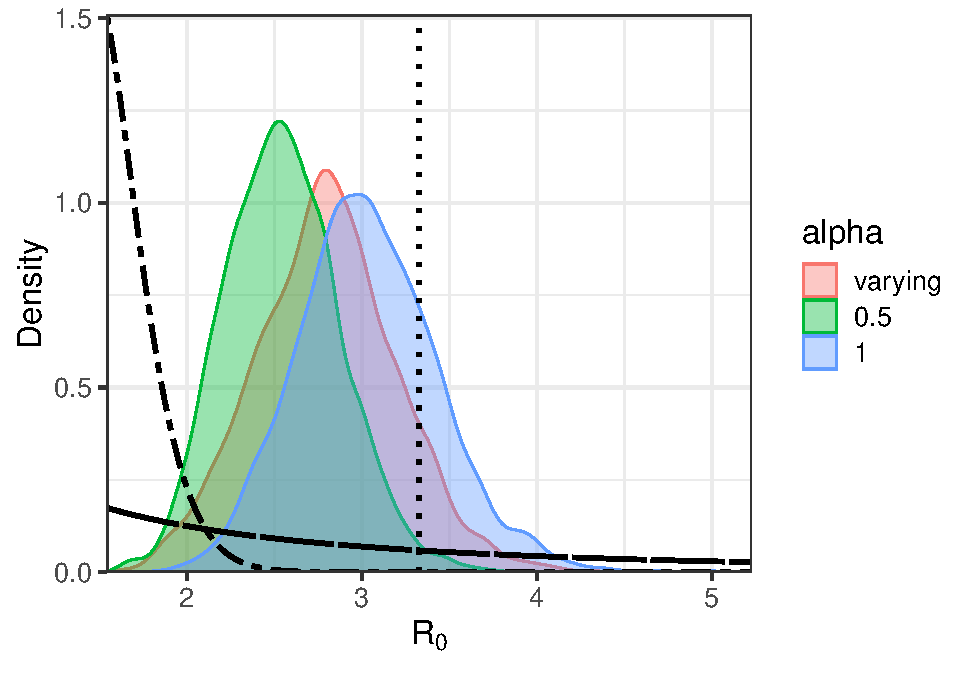
\includegraphics[scale=.32]{../plots/R0_posteriors_SIR_boardingSchool.pdf}}
\subfigure[][Predictions]{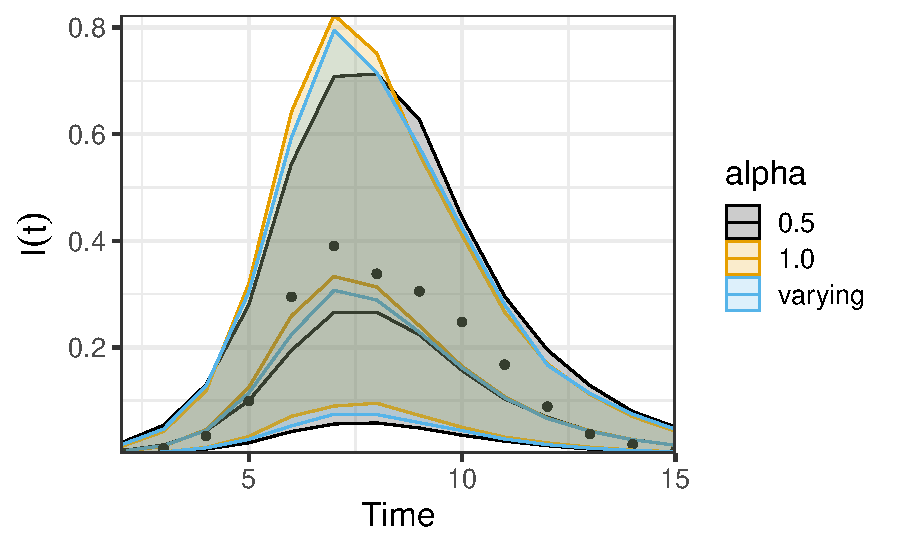
\includegraphics[scale=.35]{../plots/SIR_bands.pdf}}
\end{center}
\label{fig:SIR_results}
\end{figure}
Posterior for $\alpha$: \textbf{0.77} (0.18--0.99).
\end{frame}
%%%%%%%%%%%%%%%%%%%%%%%%%%%%%%%%%%%
%%%%%%%%%%%%%%%%%%%%%%%%%%%%%%%%%%%
\begin{frame}{Partial Sum up}
\begin{itemize}
 \item Optimality criteria often give weird results;\pause
 \item It is possible to learn about the weights from data, for some configurations of the opinions $\boldsymbol F_X$ (and the data $\boldsymbol y$);\pause
 \item Interpretation of the weights is not always straightforward;\pause
 \item In Bayesian melding, letting the pooling weight $\alpha$ vary leads to more robust inferences.
 \end{itemize}
\end{frame}
%%%%%%%%%%%%%%%%%%%%%%%%%%%%%%%%%%%
%%%%%%%%%%%%%%%%%%%%%%%%%%%%%%%%%%%
\begin{frame}{Induce-then-pool or pool-then-induce?}
\textbf{Question:} what to do when $M : \Theta \to \Phi$ is non-invertible?
We may want to gain insight about $\phi$, even though we only have expert opinions on $\theta$.
\begin{itemize}
 \item[\ding{212}] If we apply $M(\cdot)$ to each component of $\mathbf{F_\theta}$, we get a set induced distributions $\boldsymbol G_\phi$, which are then pooled to get $\pi_P(\phi)$ [\textbf{induce-then-pool}];\pause
 \item[\ding{212}] Alternatively, we can combine the $f_i(\theta)$ to obtain $\pi_T(\theta)$ and then transform to get a distribution $\pi_P^\prime(\phi)$ [\textbf{pool-then-induce}];\pause
 \item \textbf{Remark:} if $M(\cdot)$ is invertible, $\pi_P(\phi) \equiv \pi_P^\prime(\phi)$. \pause
 \item When $M$ is non-invertible, things get complicated, as we shall see.
\end{itemize}
\end{frame}
%%%%%%%%%%%%%%%%%%%%%%%%%%%%%%%%%%%
%%%%%%%%%%%%%%%%%%%%%%%%%%%%%%%%%%%
\begin{frame}{SIR model (again)}
Recall that $\theta = \{\beta, \gamma \}$ and $M(\theta) = R_0$.
Suppose $p(\beta, \gamma) = p(\beta)p(\gamma)$.
\begin{center}
 \textbf{Useful result:}
\end{center}
If $\beta \sim \text{Gamma}(k_\beta, t_\beta)$ and $\gamma \sim \text{Gamma}(k_\gamma, t_\gamma)$, then 
\begin{equation*}
\label{eq:density}
f_{R_0}(r \mid k_{\beta}, t_{\beta},  k_{\gamma}, t_{\gamma}, N ) =  \frac{(Nt_{\beta}t_{\gamma})^{k1+k2}}{\mathcal{B}(k_{\beta}, k_{\gamma})(Nt_{\beta})^{k_{\beta}}t_{\gamma}^{k_{\gamma}} } R_0^{k_{\beta}-1} (t_{\gamma} R_0 + Nt_{\beta})^{-(k_{\beta} + k_{\gamma})}
\end{equation*}
where $\mathcal{B}(a, b) = \Gamma(a + b)/\Gamma(a)\Gamma(b)$ is the Beta function.
\end{frame}
%%%%%%%%%%%%%%%%%%%%%%%%%%%%%%%%%%%
%%%%%%%%%%%%%%%%%%%%%%%%%%%%%%%%%%%
\begin{frame}{SIR model -- Priors}
\begin{figure}
\subfigure[][]{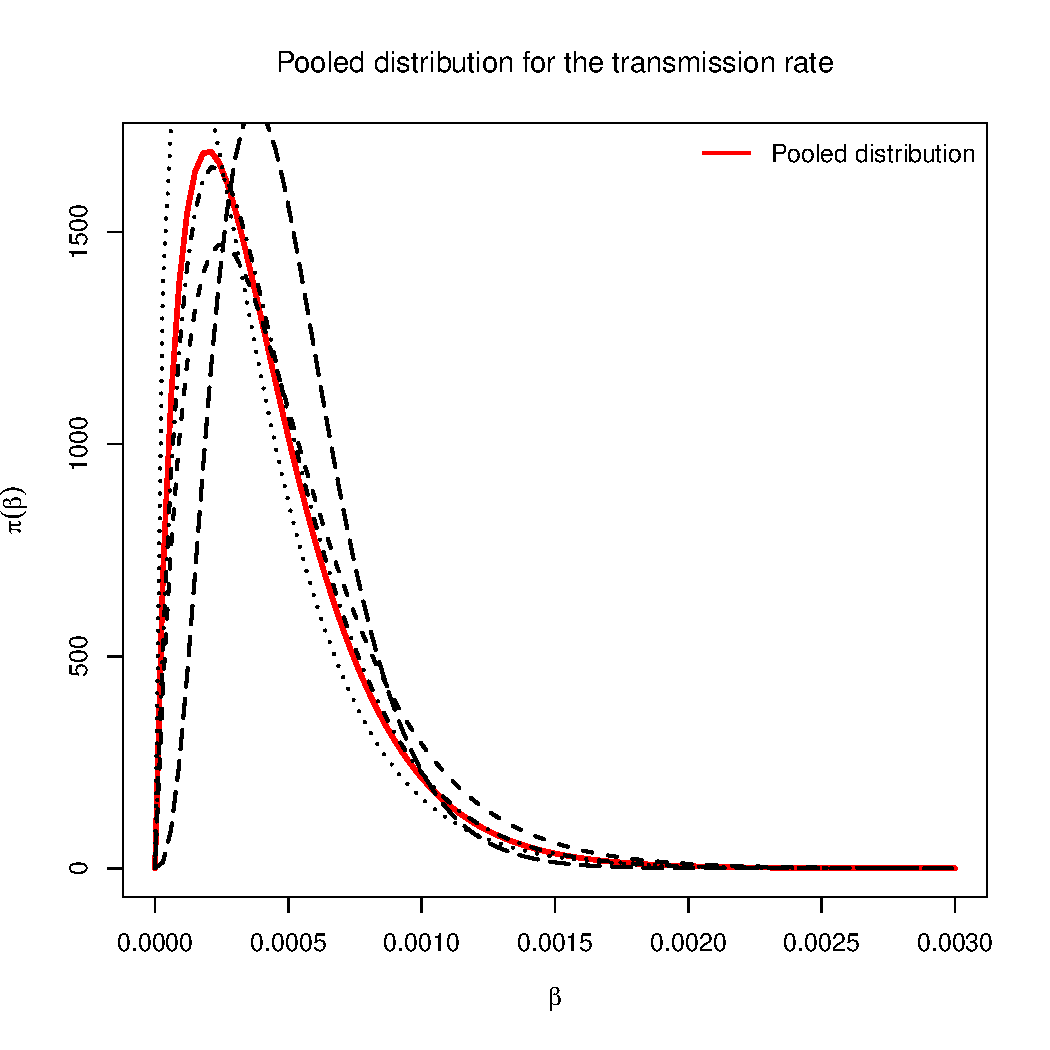
\includegraphics[scale=0.30]{figures/minKL_infection.pdf}} 
\subfigure[][]{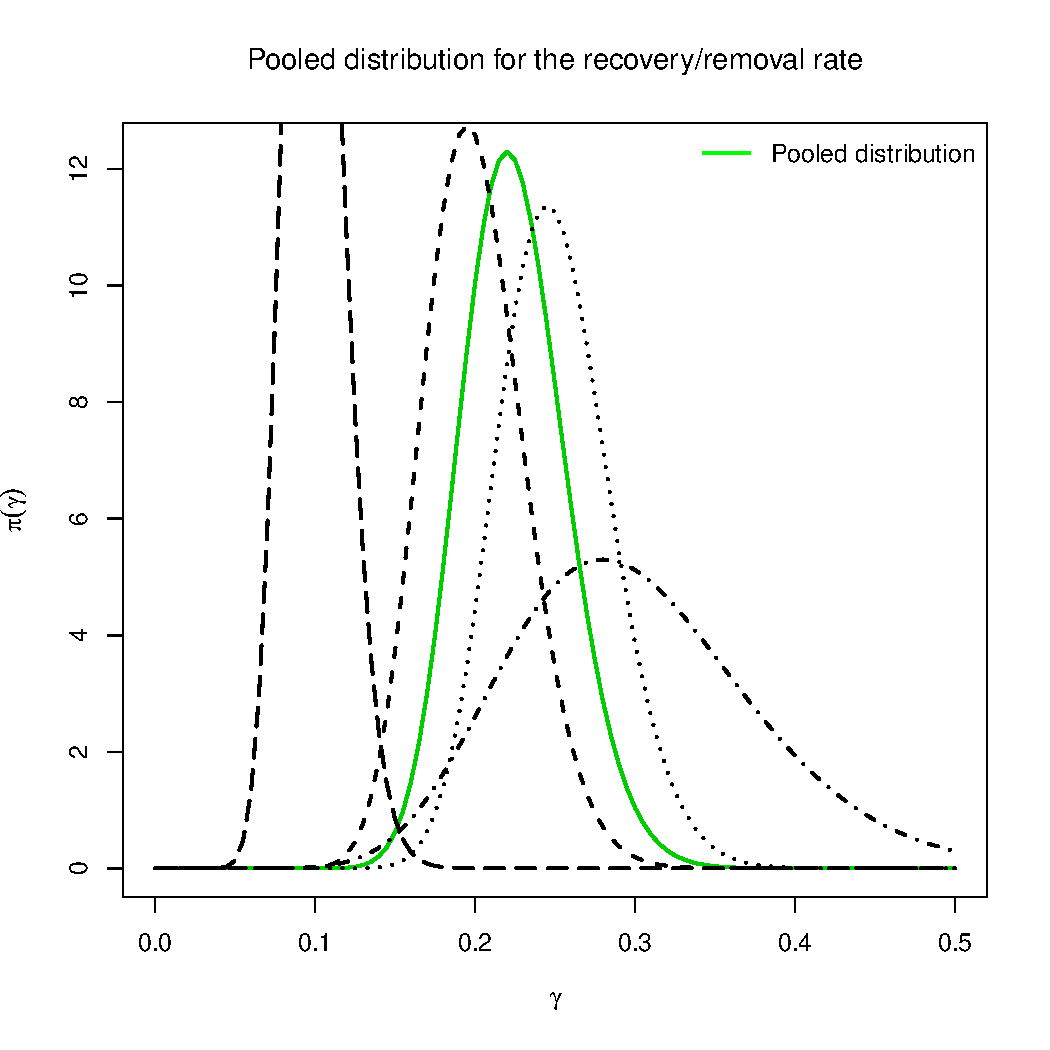
\includegraphics[scale=0.30]{figures/minKL_recovery.pdf}} 
\end{figure}
\end{frame}
%%%%%%%%%%%%%%%%%%%%%%%%%%%%%%%%%%%
%%%%%%%%%%%%%%%%%%%%%%%%%%%%%%%%%%%
\begin{frame}{Pool-then-induce}
\begin{itemize}
 \item Pool:
 \[ \pi(\beta) = Gamma(t_{1}^*, k_{1}^*) \]
 \[ \pi(\gamma) = Gamma(t_{2}^*, k_{2}^*) \]
 where $t^* = \sum_{i= 0}^K \alpha_i t_i$ and $k^* = \sum_{i= 0}^K \alpha_i k_i$.
Then
\item Induce:
\[ \pi(R_0) \propto  {R_0}^{k_1-1} (t_{2}^* R_0 + Nt_{1}^*)^{-(k_{1}^* +  k_{2}^*)}\]
\item Nice! 
\end{itemize}
\end{frame}
%%%%%%%%%%%%%%%%%%%%%%%%%%%%%%%%%%%
%%%%%%%%%%%%%%%%%%%%%%%%%%%%%%%%%%%
\begin{frame}{Induce-then-pool}
\begin{itemize}
 \item Induce (transform) each distribution (Gamma ratio):
 \[ g_{i}(R_0) \propto  {R_0}^{k_1-1} (t_2 R_0 + Nt_1)^{-(k_1 + k_2)} \]
 then
\item Pool:
\[ \pi^\prime(R_0)  \propto \prod_{i = 0}^K g_{i}(R_0) ^{\alpha_i}\]
\item Ugly!
\end{itemize}
\end{frame}
%%%%%%%%%%%%%%%%%%%%%%%%%%%%%%%%%%%
%%%%%%%%%%%%%%%%%%%%%%%%%%%%%%%%%%%
\begin{frame}{Pool-then-induce~\textit{vs} Induce-then-pool}
 \begin{figure}
 \begin{center}
  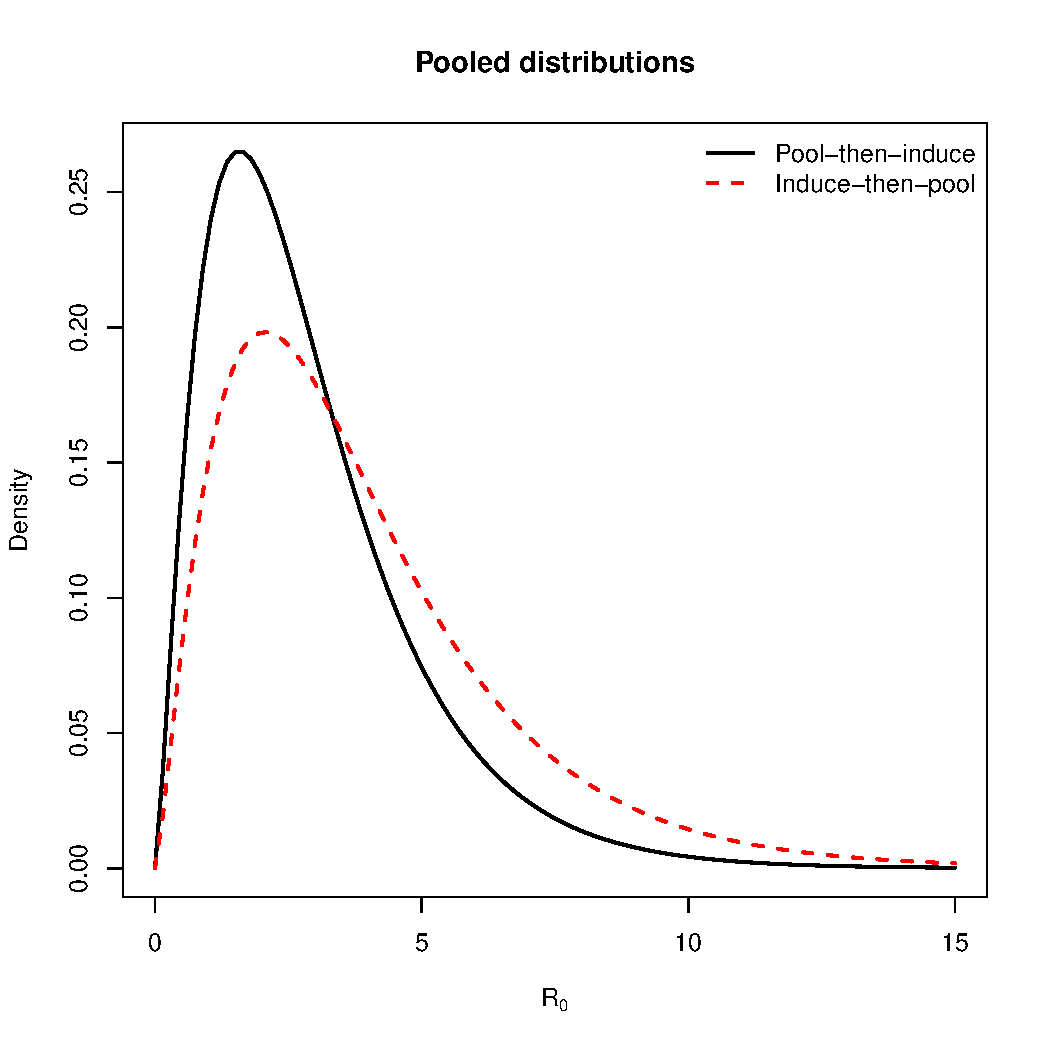
\includegraphics[scale=0.4]{figures/ItP_vs_PtI_equalWeights.pdf}
 \end{center}
  \end{figure}
\end{frame}
%%%%%%%%%%%%%%%%%%%%%%%%%%%%%%%%%%%
%%%%%%%%%%%%%%%%%%%%%%%%%%%%%%%%%%%
\begin{frame}{A final result}
\begin{remark}
 \label{rmk:invertibleIFF}
 It is possible to have  $\pi_\Phi \equiv \pi_\Phi^{\prime}$ even when $M$ is not invertible.
\end{remark}
\begin{proof}
 By an explict example. 
 Let $\theta \sim \text{normal}(0, \sigma^2)$ and let $M(\theta) = \theta^2$.
 If we define $\Omega(\phi) := \{ x: M(x) = \phi \}$ then clearly $\Omega(\phi) = \{ \omega_0, \omega_1 \} = \{ -\sqrt{\phi}, \sqrt{\phi} \}$ and hence
 \begin{align*}
 \label{eq:normalInvert}
 g_i(\phi) &= \frac{f_i(\omega_0)}{|2\omega_0|} + \frac{f_i(\omega_1)}{|2\omega_1|}, \\
        &= \frac{f_i(\sqrt{\phi})}{\sqrt{\phi}} = \frac{1}{\sqrt{2\pi v_i \phi}} \exp\left(-\frac{\phi}{2v_i}\right),
\end{align*}
where the second line follows by using the symmetry of $f_i$ around zero.
Rest of the proof follows analogously to the arguments in~\cite{Carvalho2019} for the pool of Gaussians.
\end{proof}
\end{frame}
%%%%%%%%%%%%%%%%%%%%%%%%%%%%%%%%%%%
%%%%%%%%%%%%%%%%%%%%%%%%%%%%%%%%%%%
\begin{frame}{Take home}
\begin{itemize}[label={$\tau_h$}]
 \item Log-linear mixtures have many desirable properties;\pause
 \item It is possible to learn the weights from data, under certain constraints;\pause
 \item Letting the weights vary can lead to more flexible prior modelling and better posterior inferences;\pause
 \item Further work is needed in order to make logarithmic pooling widely applicable in Statistics.
\end{itemize}
\end{frame}
%%%%%%%%%%%%%%%%%%%%%%%%%%%%%%%%%%%
%%%%%%%%%%%%%%%%%%%%%%%%%%%%%%%%%%%
\begin{frame}{Thank you!}
 \begin{itemize}
  \item Thank you very much for your attention!
  \item The authors would like to thank Professor Adrian Raftery (University of Washington) for helpful suggestions.
DAMV was supported in part by Capes under Capes/Cofecub project (N. 833/15).
FCC is grateful to Funda\c{c}\~ao Getulio Vargas for funding during this project.
  \item All the necessary code and data are publicly available at~\url{https://github.com/maxbiostat/opinion_pooling}
 \end{itemize}
\end{frame}
